\subsection{Récurrent (RNN)}
\subsubsection*{Structure}
\begin{figure}
 \centering
 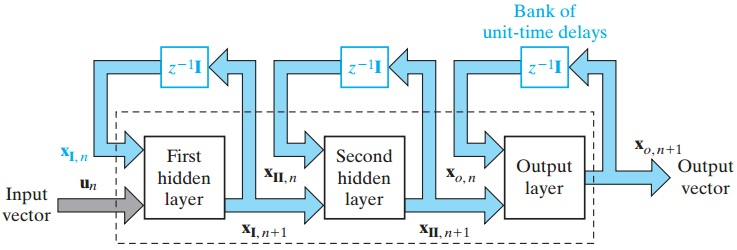
\includegraphics[scale=0.5]{../figures/structurermlp.jpg}
 \caption{Structure RLMP. \textbf{Source}: Haykin. p795\cite{Haykin}}
 \label{structurermlp}
\end{figure}
\begin{figure}
 \centering
 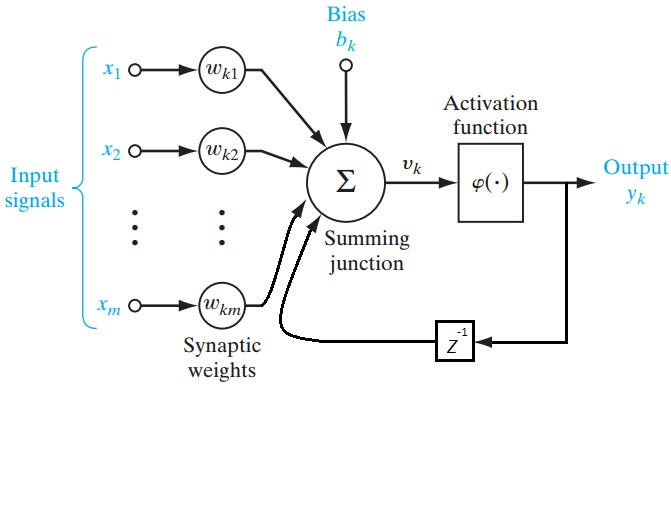
\includegraphics[scale=0.5]{../figures/neuronermlp.jpg}
 \caption{Neurone caché d'un RMLP}
 \label{neuronermlp}
\end{figure}
Un réseau de neurones récurrent est un réseaux présentant des boucles dans sa structure.
Des \emph{délais} notés $Z^{-1}$ sont présents sur certains arcs dans le réseau afin de retarder d'une étape, la transmission d'une valeur.
Une étape dans un réseau consiste à recevoir une entrée et de générer une sortie.
Il existe plusieurs réseaux de type récurrent (récurrent simple, machine à états liquide, etc).
La Figure \ref{structurermlp} présente un réseau de type perceptron multi-couches récurrent (\rmlp).
Il s'agit d'un \mlp dont les neurones des couches cachées ont un arc qui boucle sur le neurone lui-même avec un $Z^{-1}$ sur cet arc, comme sur la Figure \ref{neuronermlp}.
\subsubsection*{Applications}
Grâce aux délais, le réseau peut approximer des fonctions dont la sortie ne dépend pas seulement de l'entrée actuelle mais aussi des entrées précédentes.
Par exemple, le réseau de neurones récurrent simple (\srn), qui est un \rmlp à une seule couche cachée, peu déja effectuer des prédictions de symbole en suivant une séquence.
%Les \emph{machines à états liquides} (\lsm), dont les connections se font de manière aléàtoire, sont utilisés pour la reconnaissance automatique de la parole. %TODO citer
%Les \emph{long-short term memory} sont utilisés pour la reconnaissance automatique de la parole ou de l'écriture manuscrite. %TODO citer